\documentclass[aspectratio=169]{beamer}

% Theme and color settings
\usetheme{Madrid}
\usecolortheme{default}

% Duke blue color scheme
\definecolor{DukeBlue}{RGB}{0,0,156}
\definecolor{DukeNavy}{RGB}{0,26,87}
\definecolor{LightBlue}{RGB}{57,117,175}

\setbeamercolor{structure}{fg=DukeBlue}
\setbeamercolor{palette primary}{bg=DukeBlue,fg=white}
\setbeamercolor{palette secondary}{bg=DukeNavy,fg=white}
\setbeamercolor{palette tertiary}{bg=LightBlue,fg=white}
\setbeamercolor{frametitle}{bg=DukeBlue,fg=white}
\setbeamercolor{title}{fg=white}
\setbeamercolor{block title}{bg=DukeBlue,fg=white}
\setbeamercolor{block body}{bg=LightBlue!10}

% Remove navigation symbols
\setbeamertemplate{navigation symbols}{}

% Packages
\usepackage{tikz}
\usetikzlibrary{shapes,arrows,positioning,calc,fit}
\usepackage{amsmath,amssymb}
\usepackage{graphicx}
\usepackage{booktabs}
\usepackage{array}
\usepackage{multirow}
\usepackage[backend=bibtex,style=numeric,sorting=none,maxbibnames=3]{biblatex}
\addbibresource{CS402.bib}

% Title information
\title[AI in Neuroscience]{The Development and Outlook of AI Techniques in the Field of Neuroscience}
\subtitle{COMPSCI 402 – Artificial Intelligence\\Final Presentation}
\author{Juntang Wang\thanks{jw853@duke.edu}}
\institute{Duke Kunshan University}
\date{October 13, 2025}

\begin{document}

% Slide 1: Title Slide
\begin{frame}
  \titlepage
\end{frame}

% Slide 2: Overview/Roadmap
\begin{frame}{Presentation Overview}
  \begin{enumerate}
    \item \textbf{Introduction}
    \begin{itemize}
      \item Motivation and bidirectional relationship
      \item Three main directions
    \end{itemize}
    
    \item \textbf{Related Work}
    \begin{itemize}
      \item Historical development
      \item Recent advances
    \end{itemize}
    
    \item \textbf{Methodology: Taxonomy of AI in Neuroscience}
    \begin{itemize}
      \item Neural decoding \& brain-computer interfaces
      \item Disease diagnosis \& neuroimaging
      \item Neuroscience-inspired AI architectures
    \end{itemize}
    
    \item \textbf{Results \& Discussion}
    
    \item \textbf{Conclusion \& Future Directions}
  \end{enumerate}
\end{frame}

% Slide 3: Motivation
\begin{frame}{Motivation: A Bidirectional Relationship}
  \begin{columns}[T]
    \begin{column}{0.5\textwidth}
      \textbf{AI $\rightarrow$ Neuroscience}
      \begin{itemize}
        \item Decode brain states
        \item Analyze neural signals
        \item Model brain responses
        \item Enable brain-computer interfaces
        \item Diagnose neurological disorders
      \end{itemize}
    \end{column}
    
    \begin{column}{0.5\textwidth}
      \textbf{Neuroscience $\rightarrow$ AI}
      \begin{itemize}
        \item Inspire new architectures
        \item Guide learning algorithms
        \item Improve energy efficiency
        \item Enhance biological plausibility
        \item Drive neuromorphic computing
      \end{itemize}
    \end{column}
  \end{columns}
  
  \vspace{1em}
  \begin{center}
    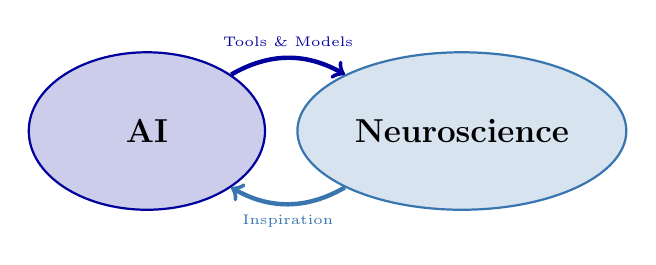
\begin{tikzpicture}
      \node[ellipse, draw=DukeBlue, thick, minimum width=3cm, minimum height=2cm, fill=DukeBlue!20] (ai) at (0,0) {\large\textbf{AI}};
      \node[ellipse, draw=LightBlue, thick, minimum width=3cm, minimum height=2cm, fill=LightBlue!20] (neuro) at (4,0) {\large\textbf{Neuroscience}};
      \draw[->,ultra thick,DukeBlue] (ai.north east) to[bend left=30] node[above] {\tiny Tools \& Models} (neuro.north west);
      \draw[->,ultra thick,LightBlue] (neuro.south west) to[bend left=30] node[below] {\tiny Inspiration} (ai.south east);
    \end{tikzpicture}
  \end{center}
  
  \tiny \cite{onciulArtificialIntelligenceNeuroscience2025,hassabisNeuroscienceinspiredArtificialIntelligence2017}
\end{frame}

% Slide 4: Key Concepts & Definitions
\begin{frame}{Key Concepts: Bringing Everyone on the Same Page}
  \begin{columns}[T]
    \begin{column}{0.48\textwidth}
      \textbf{Core Terms:}
      \begin{itemize}
        \item \textbf{AI (Artificial Intelligence):}\\
        {\small Systems that learn from data to make decisions}
        
        \item \textbf{Neuroscience:}\\
        {\small Study of the nervous system and brain}
        
        \item \textbf{BCI (Brain-Computer Interface):}\\
        {\small Direct communication pathway between brain and external devices}
      \end{itemize}
    \end{column}
    
    \begin{column}{0.48\textwidth}
      \textbf{Neural Recording Methods:}
      \begin{itemize}
        \item \textbf{EEG (Electroencephalography):}\\
        {\small Records electrical brain activity via scalp electrodes}
        
        \item \textbf{fMRI (Functional MRI):}\\
        {\small Images brain activity by detecting blood flow changes}
        
        \item \textbf{Neuromorphic Computing:}\\
        {\small Hardware that mimics biological neural networks}
      \end{itemize}
    \end{column}
  \end{columns}
\end{frame}

% Slide 5: Three Directions & Key Challenges
\begin{frame}{Three Directions \& Key Challenges}
  \begin{columns}[T]
    \begin{column}{0.55\textwidth}
      \textbf{Three Main Directions:}
      \begin{enumerate}
        \item \textbf{Neural Decoding \& BCIs}\\
        {\small Extract information from neural signals}
        
        \item \textbf{Disease Diagnosis}\\
        {\small AI-powered neuroimaging analysis}
        
        \item \textbf{Neuroscience-Inspired AI}\\
        {\small Spiking networks, neuromorphic computing}
      \end{enumerate}
    \end{column}
    
    \begin{column}{0.43\textwidth}
      \textbf{Key Challenges:}
      \begin{itemize}
        \item Data complexity
        \item Multimodal integration
        \item Interpretability
        \item Generalizability
        \item Ethics \& privacy
      \end{itemize}
      
      \vspace{0.5em}
      
      \textit{\small Focus: Recent advances\\(past 5 years)}
    \end{column}
  \end{columns}
\end{frame}

% Slide 6: Evolution & Current State
\begin{frame}{From Perceptrons to Deep Learning}
  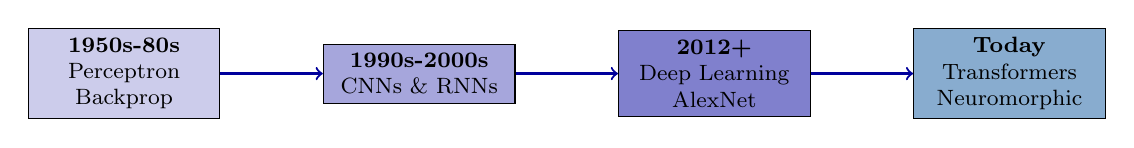
\begin{tikzpicture}[
    node distance=1.3cm,
    every node/.style={font=\footnotesize},
    arrow/.style={->,thick,DukeBlue}
  ]
    \node[rectangle, draw, fill=DukeBlue!20, text width=2.2cm, align=center] (1950s) {\textbf{1950s-80s}\\Perceptron\\Backprop};
    \node[rectangle, draw, fill=DukeBlue!35, text width=2.2cm, align=center, right=of 1950s] (1990s) {\textbf{1990s-2000s}\\CNNs \& RNNs};
    \node[rectangle, draw, fill=DukeBlue!50, text width=2.2cm, align=center, right=of 1990s] (2012) {\textbf{2012+}\\Deep Learning\\AlexNet};
    \node[rectangle, draw, fill=LightBlue!60, text width=2.2cm, align=center, right=of 2012] (now) {\textbf{Today}\\Transformers\\Neuromorphic};
    
    \draw[arrow] (1950s) -- (1990s);
    \draw[arrow] (1990s) -- (2012);
    \draw[arrow] (2012) -- (now);
  \end{tikzpicture}
  
  \vspace{0.8em}
  
  \begin{columns}[T]
    \begin{column}{0.48\textwidth}
      \textbf{Major Achievements:}
      \begin{itemize}
        \item Visual reconstruction from fMRI
        \item Expert-level disease detection
        \item Neuromorphic hardware (Loihi)
        \item Real-time BCIs
      \end{itemize}
    \end{column}
    
    \begin{column}{0.48\textwidth}
      \textbf{Current Gaps:}
      \begin{itemize}
        \item No unified brain models
        \item Limited interpretability
        \item Poor generalizability
        \item Ethical frameworks needed
      \end{itemize}
    \end{column}
  \end{columns}
\end{frame}

% Slide 7: Taxonomy Overview
\begin{frame}{Taxonomy of AI in Neuroscience}
  \begin{center}
    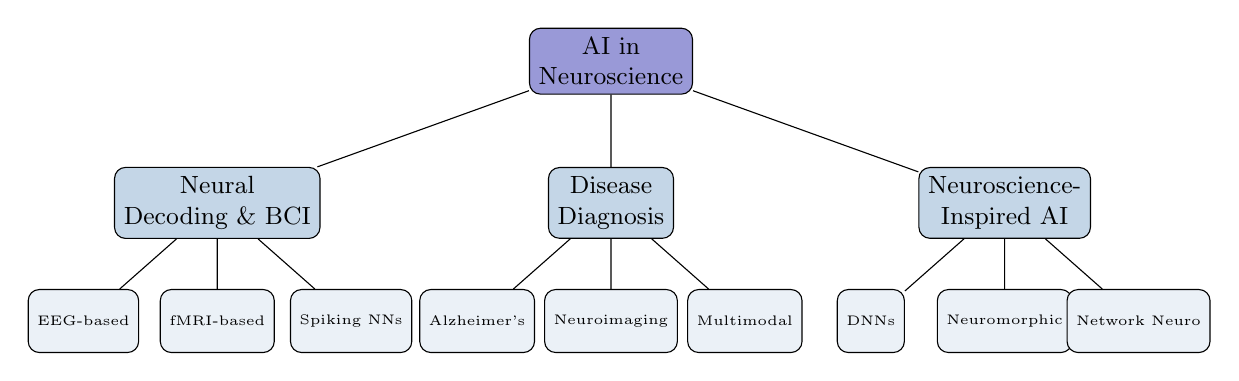
\begin{tikzpicture}[
      level 1/.style={sibling distance=5cm, level distance=1.8cm},
      level 2/.style={sibling distance=1.7cm, level distance=1.5cm},
      every node/.style={rectangle, draw, rounded corners, font=\small, align=center, minimum height=0.8cm},
      root/.style={fill=DukeBlue!40},
      category/.style={fill=LightBlue!30},
      subcategory/.style={fill=LightBlue!10, font=\tiny}
    ]
      \node[root] {AI in\\Neuroscience}
        child {node[category] {Neural\\Decoding \& BCI}
          child {node[subcategory] {EEG-based}}
          child {node[subcategory] {fMRI-based}}
          child {node[subcategory] {Spiking NNs}}
        }
        child {node[category] {Disease\\Diagnosis}
          child {node[subcategory] {Alzheimer's}}
          child {node[subcategory] {Neuroimaging}}
          child {node[subcategory] {Multimodal}}
        }
        child {node[category] {Neuroscience-\\Inspired AI}
          child {node[subcategory] {DNNs}}
          child {node[subcategory] {Neuromorphic}}
          child {node[subcategory] {Network Neuro}}
        };
    \end{tikzpicture}
  \end{center}
\end{frame}

% Slide 8: Category 1 - Neural Decoding
\begin{frame}{Category 1: Neural Decoding \& Brain-Computer Interfaces}
  \textbf{Electroencephalography (EEG) Approaches}
  \begin{itemize}
    \item \textbf{EEGNet:} Compact CNN for EEG-based BCIs \cite{lawhernEEGNetCompactConvolutional2018}
    % \begin{itemize}
    %   \item Depthwise and separable convolutions
    %   \item Superior generalization across paradigms
    %   \item P300, error-related negativity, motor rhythms
    % \end{itemize}
    \item \textbf{Transformer Architectures:} Better temporal dependencies
  \end{itemize}
  
  \vspace{0.5em}
  
  \textbf{Neuroimaging (fMRI) Decoding}
  \begin{itemize}
    \item Deep neural networks reconstruct visual experiences \cite{mathisDecodingBrainNeural2024}
    \item Motion-energy encoding models
    \item Separate fast visual info from slow hemodynamic responses
  \end{itemize}
  
  \vspace{0.5em}
  
  \textbf{Spiking Neural Networks}
  \begin{itemize}
    \item \textbf{SuperSpike:} Supervised learning for integrate-and-fire neurons \cite{zenkeSuperSpikeSupervisedLearning2018}
    \item \textbf{LSTM-SNNs:} Learning-to-learn scenarios \cite{bellecLongShorttermMemory2018}
  \end{itemize}
\end{frame}

% Slide 9: Category 2 - Disease Diagnosis
\begin{frame}{Category 2: Disease Diagnosis \& Neuroimaging Analysis}
  \textbf{Alzheimer's Disease Detection}
  \begin{itemize}
    \item \textbf{AlzheimerNet:} Fine-tuned CNN \cite{shamratAlzheimerNetEffectiveDeep2023}
    % \begin{itemize}
    %   \item Identifies all 5 stages + normal controls
    %   \item 98.67\% accuracy
    %   \item Uses data augmentation \& CLAHE enhancement
    % \end{itemize}
    \item \textbf{YOLOv11:} Multimodal fusion (MRI + DTI) \cite{hechkelEarlyDetectionClassification2025}
    % \begin{itemize}
    %   \item 93.6\% precision, 91.6\% recall, 96.7\% mAP50
    %   \item Object detection architecture for medical imaging
    % \end{itemize}
  \end{itemize}
  
  \vspace{0.5em}
  
  \textbf{General Neuroimaging Analysis}
  \begin{itemize}
    \item CNNs now methodology of choice \cite{litjensSurveyDeepLearning2017}
    \item Applications: classification, detection, segmentation, registration
    \item Multimodal integration \cite{lorenziIntegrationMultimodalData2023}: neuroimaging + electrophysiology + behavior
  \end{itemize}
\end{frame}

% Slide 10: Category 3 - Neuroscience-Inspired AI
\begin{frame}{Category 3: Neuroscience-Inspired AI Architectures}
  \textbf{Deep Neural Networks as Brain Models}
  \begin{itemize}
    \item Model neural responses in ventral visual pathway \cite{gucluDeepNeuralNetworks2015}
    \item Explicit gradients for feature complexity
    \item Map stimulus features across human brain
    \item Dorsal stream representations shared between subjects
  \end{itemize}
  
  \vspace{0.5em}
  
  \textbf{Neuromorphic Computing}
  \begin{itemize}
    \item \textbf{Intel Loihi Processor:} \cite{daviesLoihiNeuromorphicManycore2018}
    % \begin{itemize}
    %   \item Neuromorphic manycore with on-chip learning
    %   \item 1000× better energy-delay-product vs CPUs
    %   \item Hierarchical connectivity, dendritic compartments
    %   \item Spike-based computation
    % \end{itemize}
  \end{itemize}
  
  \vspace{0.5em}
  
  \textbf{Network Neuroscience}
  \begin{itemize}
    \item Graph-theoretic analysis of neural connectivity \cite{bassettNetworkNeuroscience2017}
    \item Brain-inspired learning algorithms
    \item Structural and functional connectivity patterns
  \end{itemize}
\end{frame}

% Slide 11: Summary Table
\begin{frame}{Comparison of Representative Methods}
  \small
  \begin{table}
    \centering
    \begin{tabular}{l l l l}
      \toprule
      \textbf{Category} & \textbf{Method} & \textbf{Key Strength} & \textbf{Application} \\
      \midrule
      \multirow{2}{*}{Neural Decoding} 
        & EEGNet & Generalization & BCI control \\
        & Motion-energy & Reconstruction & Visual decoding \\
      \midrule
      \multirow{2}{*}{Disease Diagnosis} 
        & AlzheimerNet & 98.67\% accuracy & AD staging \\
        & YOLOv11 & Multimodal fusion & Early detection \\
      \midrule
      \multirow{2}{*}{Inspired AI} 
        & DNNs & Brain modeling & Feature mapping \\
        & Loihi & Energy efficiency & Neuromorphic \\
      \bottomrule
    \end{tabular}
  \end{table}
  
  \vspace{0.5em}
  
  \textbf{Common Considerations:}
  \begin{itemize}
    \item Choice depends on application, data modality, computational constraints
    \item Multimodal integration requires sophisticated approaches
    \item Validation needs biological plausibility \& clinical relevance
  \end{itemize}
\end{frame}

% Slide 12: Key Results
\begin{frame}{Key Results Across All Categories}
  \begin{columns}[T]
    \begin{column}{0.48\textwidth}
      \textbf{Disease Diagnosis}
      \begin{itemize}
        \item \textbf{AlzheimerNet:} \textcolor{DukeBlue}{98.67\%} accuracy
        \item Classifies 5 stages + normal
        \item \textbf{YOLOv11:} 93.6\% precision, 91.6\% recall
        \item Multimodal MRI+DTI fusion
      \end{itemize}
      
      \vspace{0.5em}
      
      \textbf{Neural Decoding}
      \begin{itemize}
        \item EEGNet: Superior BCI generalization
        \item Visual reconstruction from fMRI
        \item Real-time processing achieved
      \end{itemize}
    \end{column}
    
    \begin{column}{0.48\textwidth}
      \textbf{Neuromorphic Computing}
      \begin{itemize}
        \item \textbf{Loihi:} \textcolor{DukeBlue}{1000×} energy efficiency
        \item Spike-based computation
        \item Biological plausibility + performance
      \end{itemize}
      
      \vspace{0.5em}
      
      \textbf{Brain Models}
      \begin{itemize}
        \item DNNs model ventral pathway
        \item Shared representations across subjects
        \item Automated feature mapping
      \end{itemize}
      
      \vspace{0.5em}
      
      \textit{\small Trade-off: biological realism vs. computational efficiency}
    \end{column}
  \end{columns}
\end{frame}

% Slide 13: Challenges & Ethics
\begin{frame}{Critical Challenges \& Ethical Considerations}
  \begin{columns}[T]
    \begin{column}{0.48\textwidth}
      \textbf{Technical Challenges:}
      \begin{enumerate}
        \item \textbf{Data Complexity} \cite{onciulArtificialIntelligenceNeuroscience2025}\\
        % {\small Single neurons $\rightarrow$ whole networks}
        
        \item \textbf{Multimodal Integration} \cite{lorenziIntegrationMultimodalData2023}\\
        % {\small Heterogeneous data types}
        
        \item \textbf{Interpretability} \cite{sadeghiReviewExplainableArtificial2024}\\
        % {\small "Black box" problem}
        
        \item \textbf{Generalizability} \cite{johnsonPrecisionMedicineAI2021}\\
        % {\small Individual variability}
      \end{enumerate}
    \end{column}
    
    \begin{column}{0.48\textwidth}
      \textbf{Ethical Issues:} \cite{gordonEthicalConsiderationsUse2024}
      \begin{itemize}
        \item \textbf{Privacy \& Autonomy}
        % \begin{itemize}
        %   \item Neural signal decoding
        %   \item Thought privacy
        %   \item Brain function influence
        % \end{itemize}
        
        \item \textbf{Cognitive Enhancement}
        % \begin{itemize}
        %   \item Access inequality
        %   \item Fairness concerns
        %   \item Need for regulation
        % \end{itemize}
        
        \item \textbf{Clinical Use}
        % \begin{itemize}
        %   \item Informed consent
        %   \item Data protection
        %   \item AI role in diagnosis
        % \end{itemize}
      \end{itemize}
    \end{column}
  \end{columns}
\end{frame}

% Slide 14: Future Directions & Priorities
\begin{frame}{Future Directions \& Research Priorities}
  \begin{columns}[T]
    \begin{column}{0.48\textwidth}
      \textbf{Emerging Opportunities:}
      \begin{itemize}
        \item \textbf{Technical:}
        \begin{itemize}
          \item Real-time BCIs \cite{zhangBrainComputerInterfaces2024}
          \item Closed-loop systems
          \item Large-scale neural data analysis
        \end{itemize}
        
        \item \textbf{Neuromorphic:}
        \begin{itemize}
          \item Brain-inspired architectures \cite{schmidgallBraininspiredLearningArtificial2024}
          \item Energy-efficient computing
          \item Network neuroscience + ML \cite{bassettNetworkNeuroscience2017}
        \end{itemize}
        
        \item \textbf{Clinical:} \cite{nenningMachineLearningNeuroimaging2022}
        \begin{itemize}
          \item Neurorehabilitation
          \item Communication aids
          \item Novel treatments
        \end{itemize}
      \end{itemize}
    \end{column}
    
    \begin{column}{0.48\textwidth}
      \textbf{Research Priorities:}
      \begin{enumerate}
        \item \textbf{Explainable AI}\\
        % {\small Interpretable models, clear explanations}
        
        \item \textbf{Standardization}\\
        % {\small Metrics, benchmarks, comparison}
        
        \item \textbf{Multimodal Integration}\\
        % {\small Effective data fusion}
        
        \item \textbf{Personalized AI}\\
        % {\small Individual adaptation}
        
        \item \textbf{Ethical Frameworks}\\
        % {\small Responsible development}
      \end{enumerate}
      
      \vspace{0.3em}
      
      \textit{\small Interdisciplinary collaboration essential}
    \end{column}
  \end{columns}
\end{frame}

% Slide 15: Conclusion
\begin{frame}{Conclusion \& Final Thoughts}
  \begin{columns}[T]
    \begin{column}{0.48\textwidth}
      \textbf{Key Contributions:}
      \begin{itemize}
        \item Taxonomy of AI applications
        \item Systematic analysis of methods
        \item Challenges identified
        \item Ethical considerations
      \end{itemize}
      
      \vspace{0.5em}
      
      \textbf{Key Takeaways:}
      \begin{itemize}
        \item AI transformed neuroscience
        \item Bidirectional benefits
        \item Remarkable achievements
        \item Significant challenges remain
      \end{itemize}
    \end{column}
    
    \begin{column}{0.48\textwidth}
      \textbf{Looking Forward:}
      \begin{quote}
        \small Through interdisciplinary collaboration and ethical consideration, AI-neuroscience integration will benefit both fields and society.
      \end{quote}
      
      \vspace{1em}
      
      \textbf{Acknowledgment}\\
      {\small COMPSCI 402\\Duke Kunshan University\\Prof. Peng Sun}
      
      \vspace{1em}
      
      \begin{center}
        {\Large Thank you!}\\
        {\small Questions?}
      \end{center}
    \end{column}
  \end{columns}
\end{frame}

% Slide 16: References (Backup)
\begin{frame}[allowframebreaks]{References}
  \tiny
  \printbibliography[heading=none]
\end{frame}

\end{document}

